\documentclass{beamer}

% Tema de la presentación
\usetheme{Berlin} % Puedes cambiarlo a: Warsaw, Berlin, AnnArbor, etc.
\usepackage{graphicx}

% Información del título
\title[Creación de un dashboard para usuarios del ticket digital de Mercadona]{Creación de un dashboard para usuarios del ticket digital de Mercadona con visualización gráfica de datos: evolución de precios por producto, gastos por categoría de alimentación y ventanas temporales de gastos}
\author{Santiago Sánchez Sans}
\institute{IES Abastos}
\date{6 junio 2025} % o una fecha específica

\begin{document}
	
	% Portada
	\begin{frame}
		\titlepage
	\end{frame}
	
	% Índice
	\begin{frame}
		\frametitle{Contenido}
		\tableofcontents
	\end{frame}
	
	% Sección 1
	\section{Introducción}
	
	\begin{frame}
		\frametitle{Introducción}
		Aquí va el contenido de la introducción.
		\begin{itemize}
			\item Punto 1
			\item Punto 2
			\item Punto 3
		\end{itemize}
	\end{frame}
	
	% Sección 2
	\section{Diseño}
	
	
	% DIAPO DIAGRAMA DE SISTEMES GENERAL
	\begin{frame}
		\frametitle{Diagrama de sistemas}
		 

		\begin{figure}
			\centering
			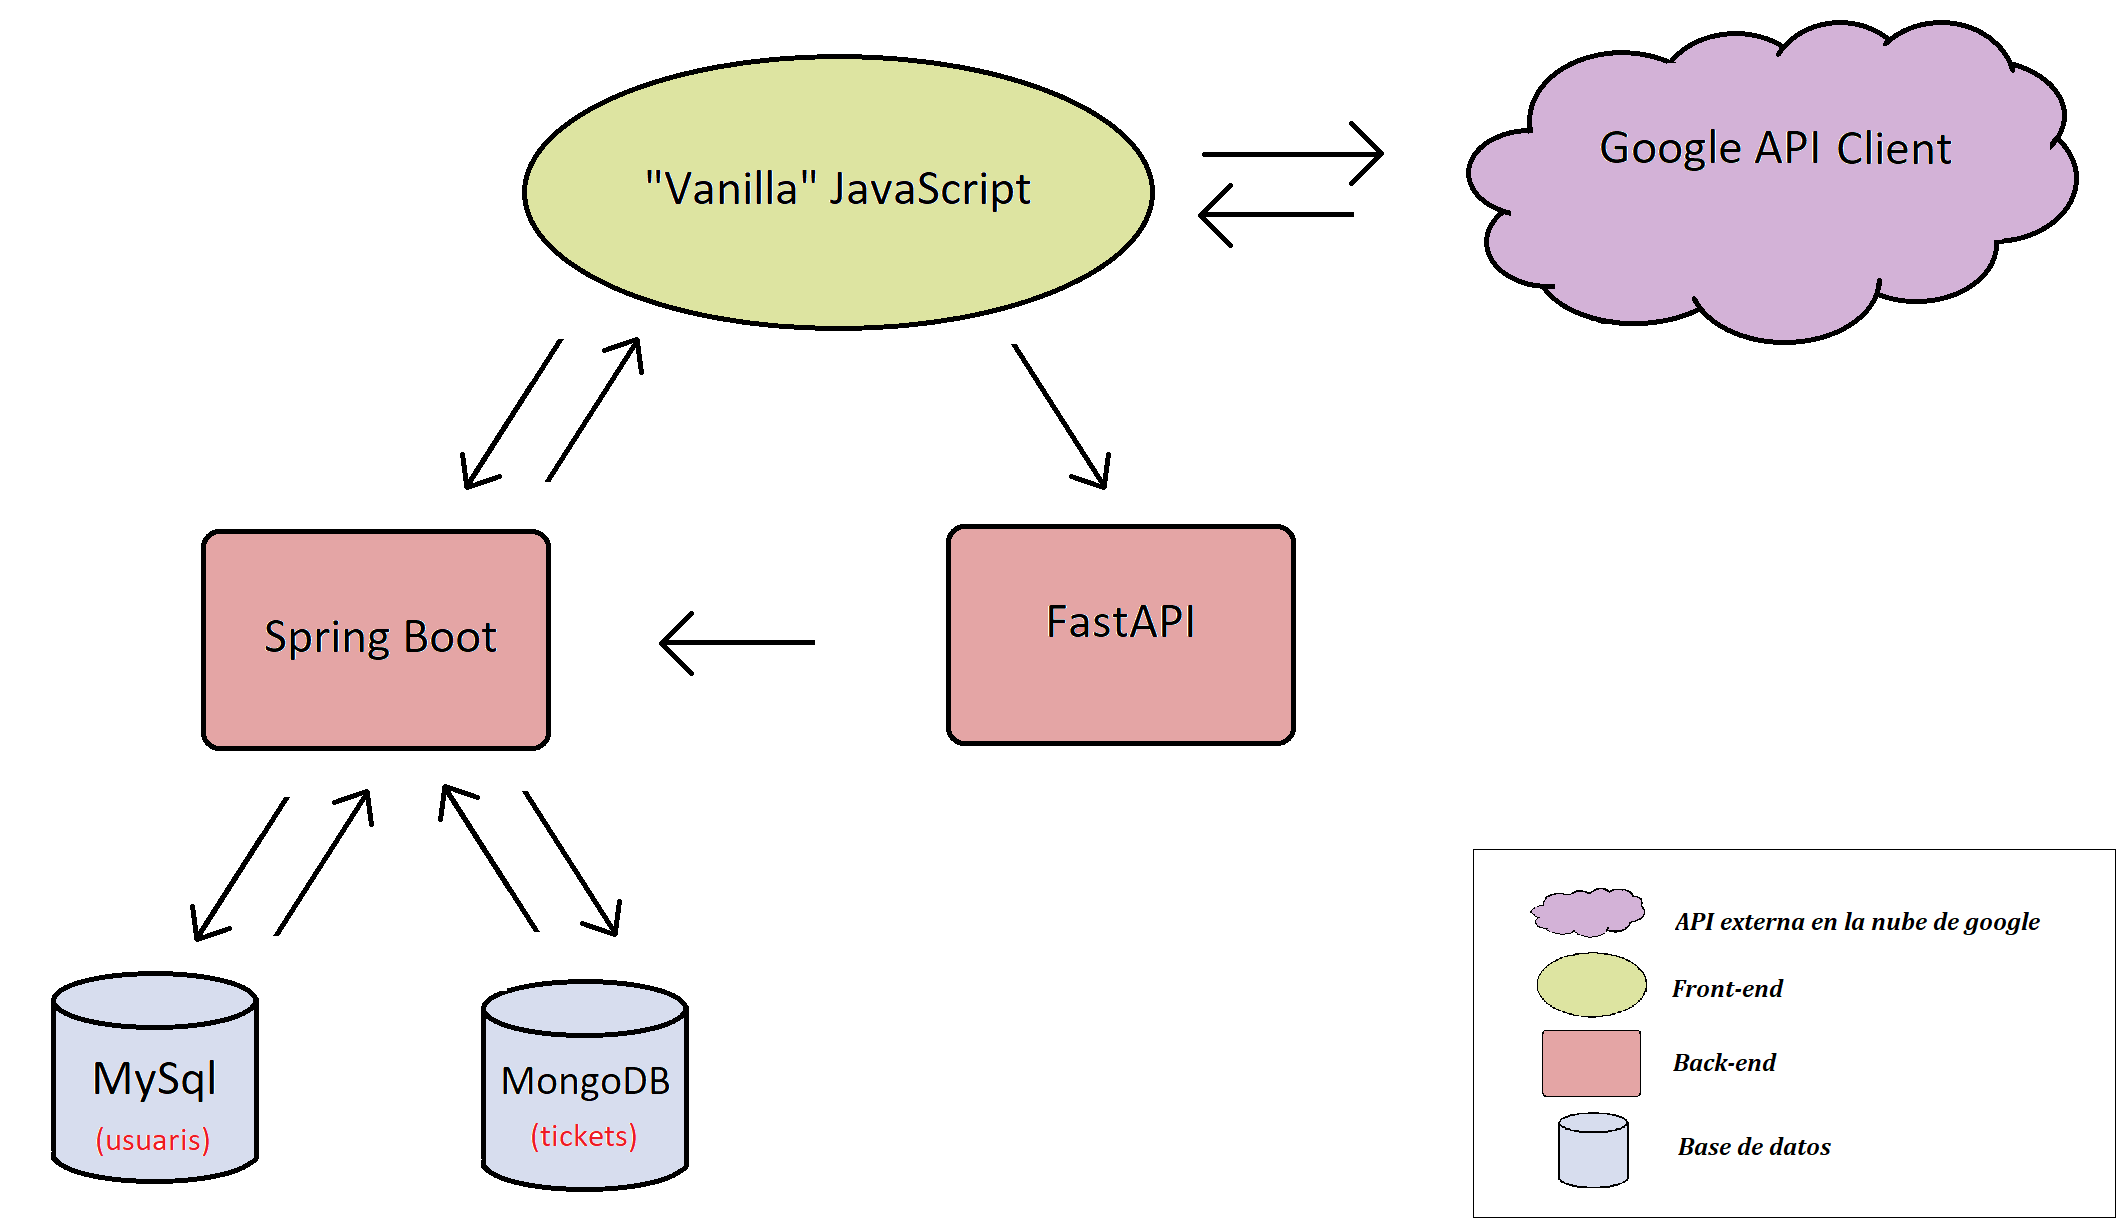
\includegraphics[width=1\linewidth]{../img/diagramaSistemesAplicacioMercapp}
			
			\label{fig:diagramasistemesaplicaciomercapp}
		\end{figure}
		
	\end{frame}
	
	
	% DIAPO DIAGRAMA SISTEMES: REGISTRE (SIMPLIFICAT)
	\begin{frame}
		\frametitle{Diagrama de sistemas: registro}
		
		\begin{figure}
			\centering
			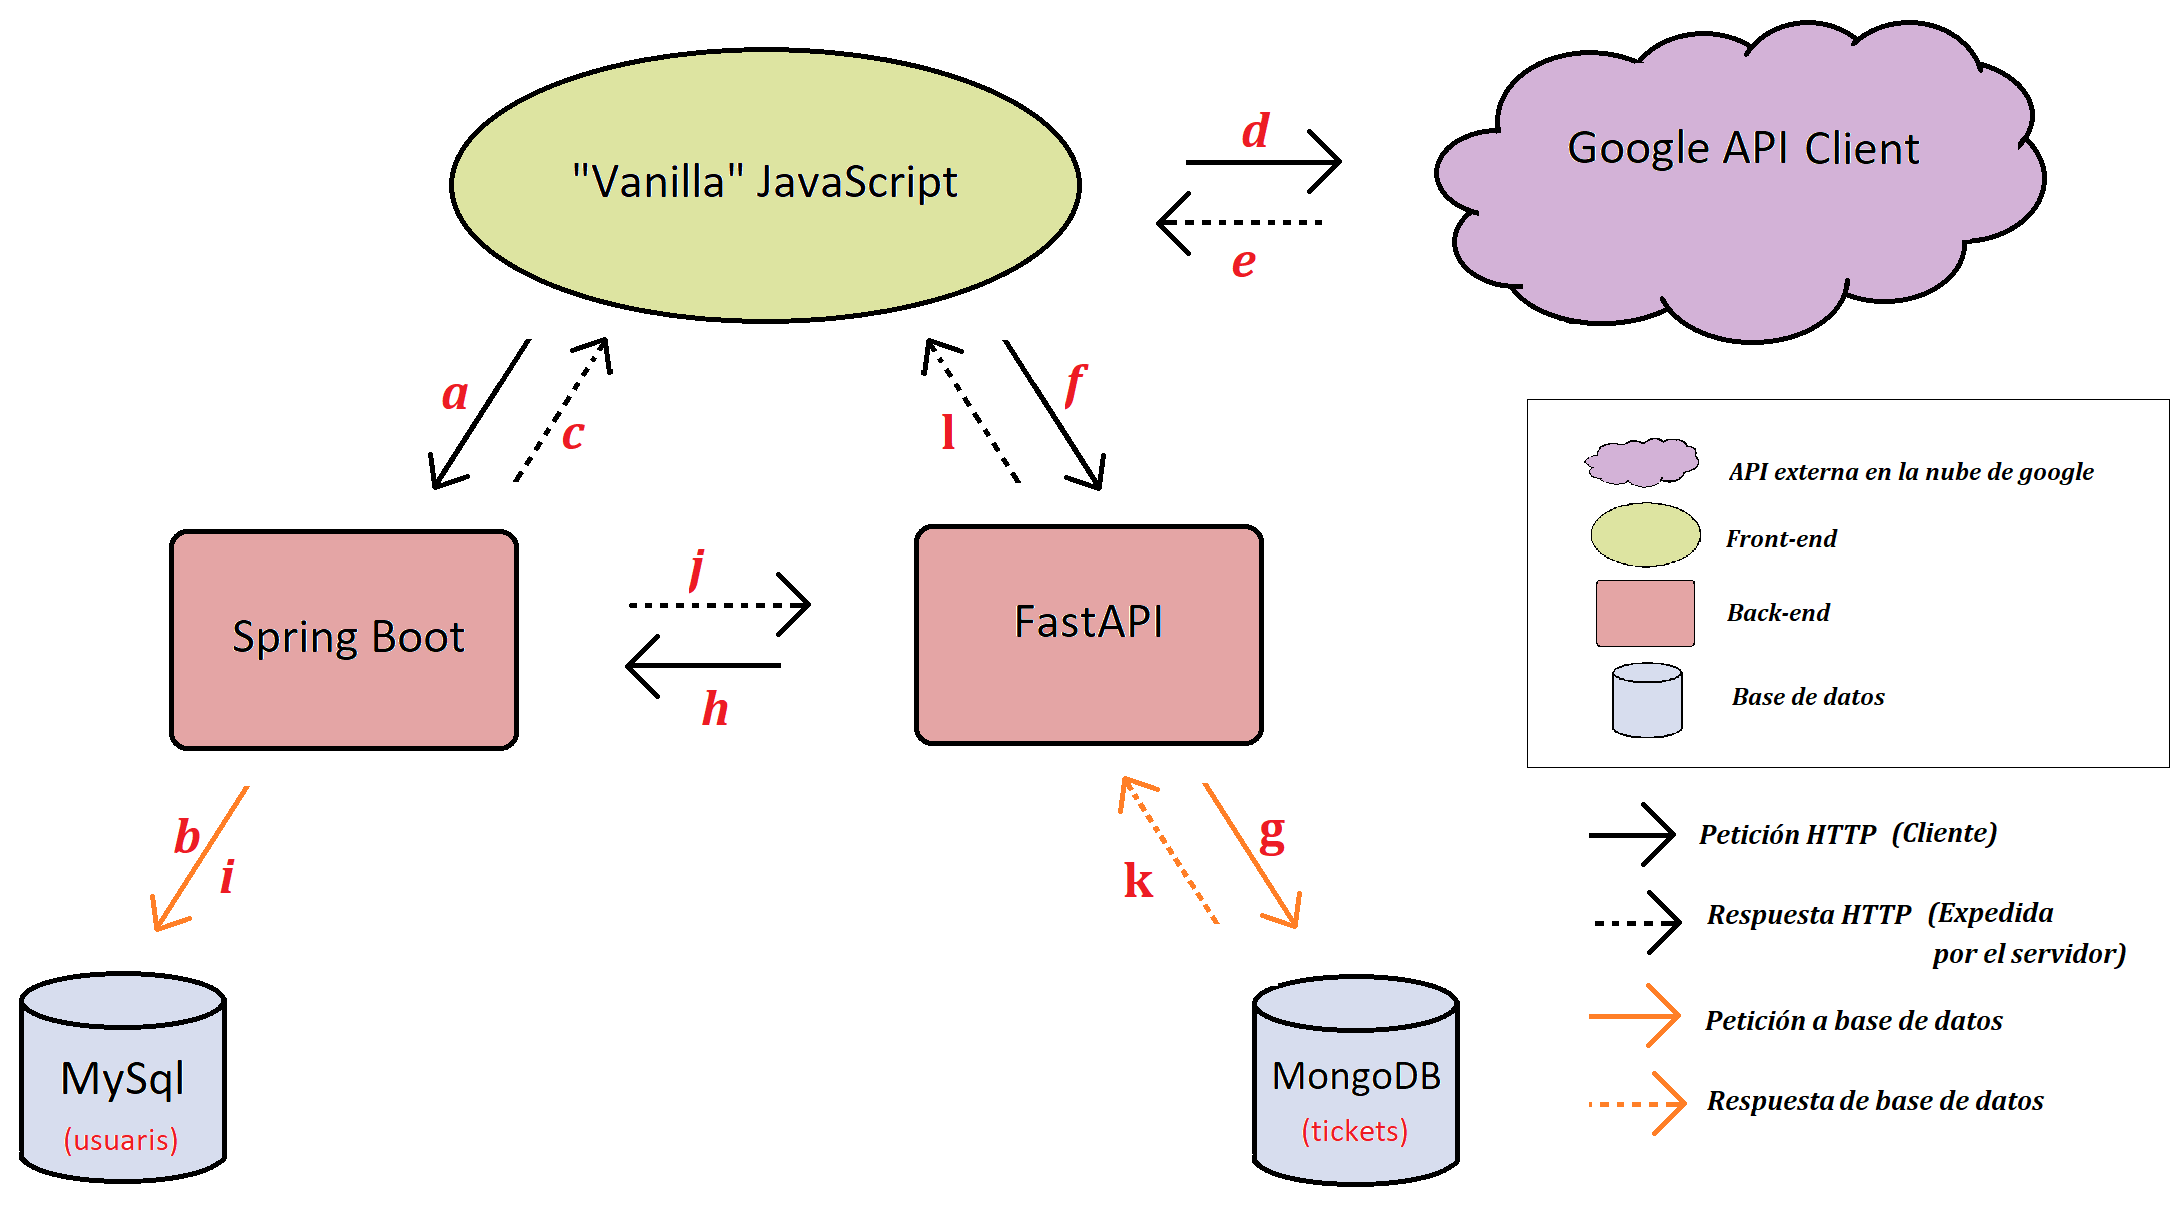
\includegraphics[width=1\linewidth]{../img/diagramaSistemesAplicacioMercappCAMIREGISTREbo}
			
			\label{fig:diagramasistemesaplicaciomercappcamiregistrebo}
		\end{figure}
		
	\end{frame}
	
	
	% DIAPO DIAGRAMA SISTEMES: REGISTRE (INICI SESSIÓ)
	\begin{frame}
		\frametitle{Diagrama de sistemas: inicio de sesión}
		
		\begin{figure}
			\centering
			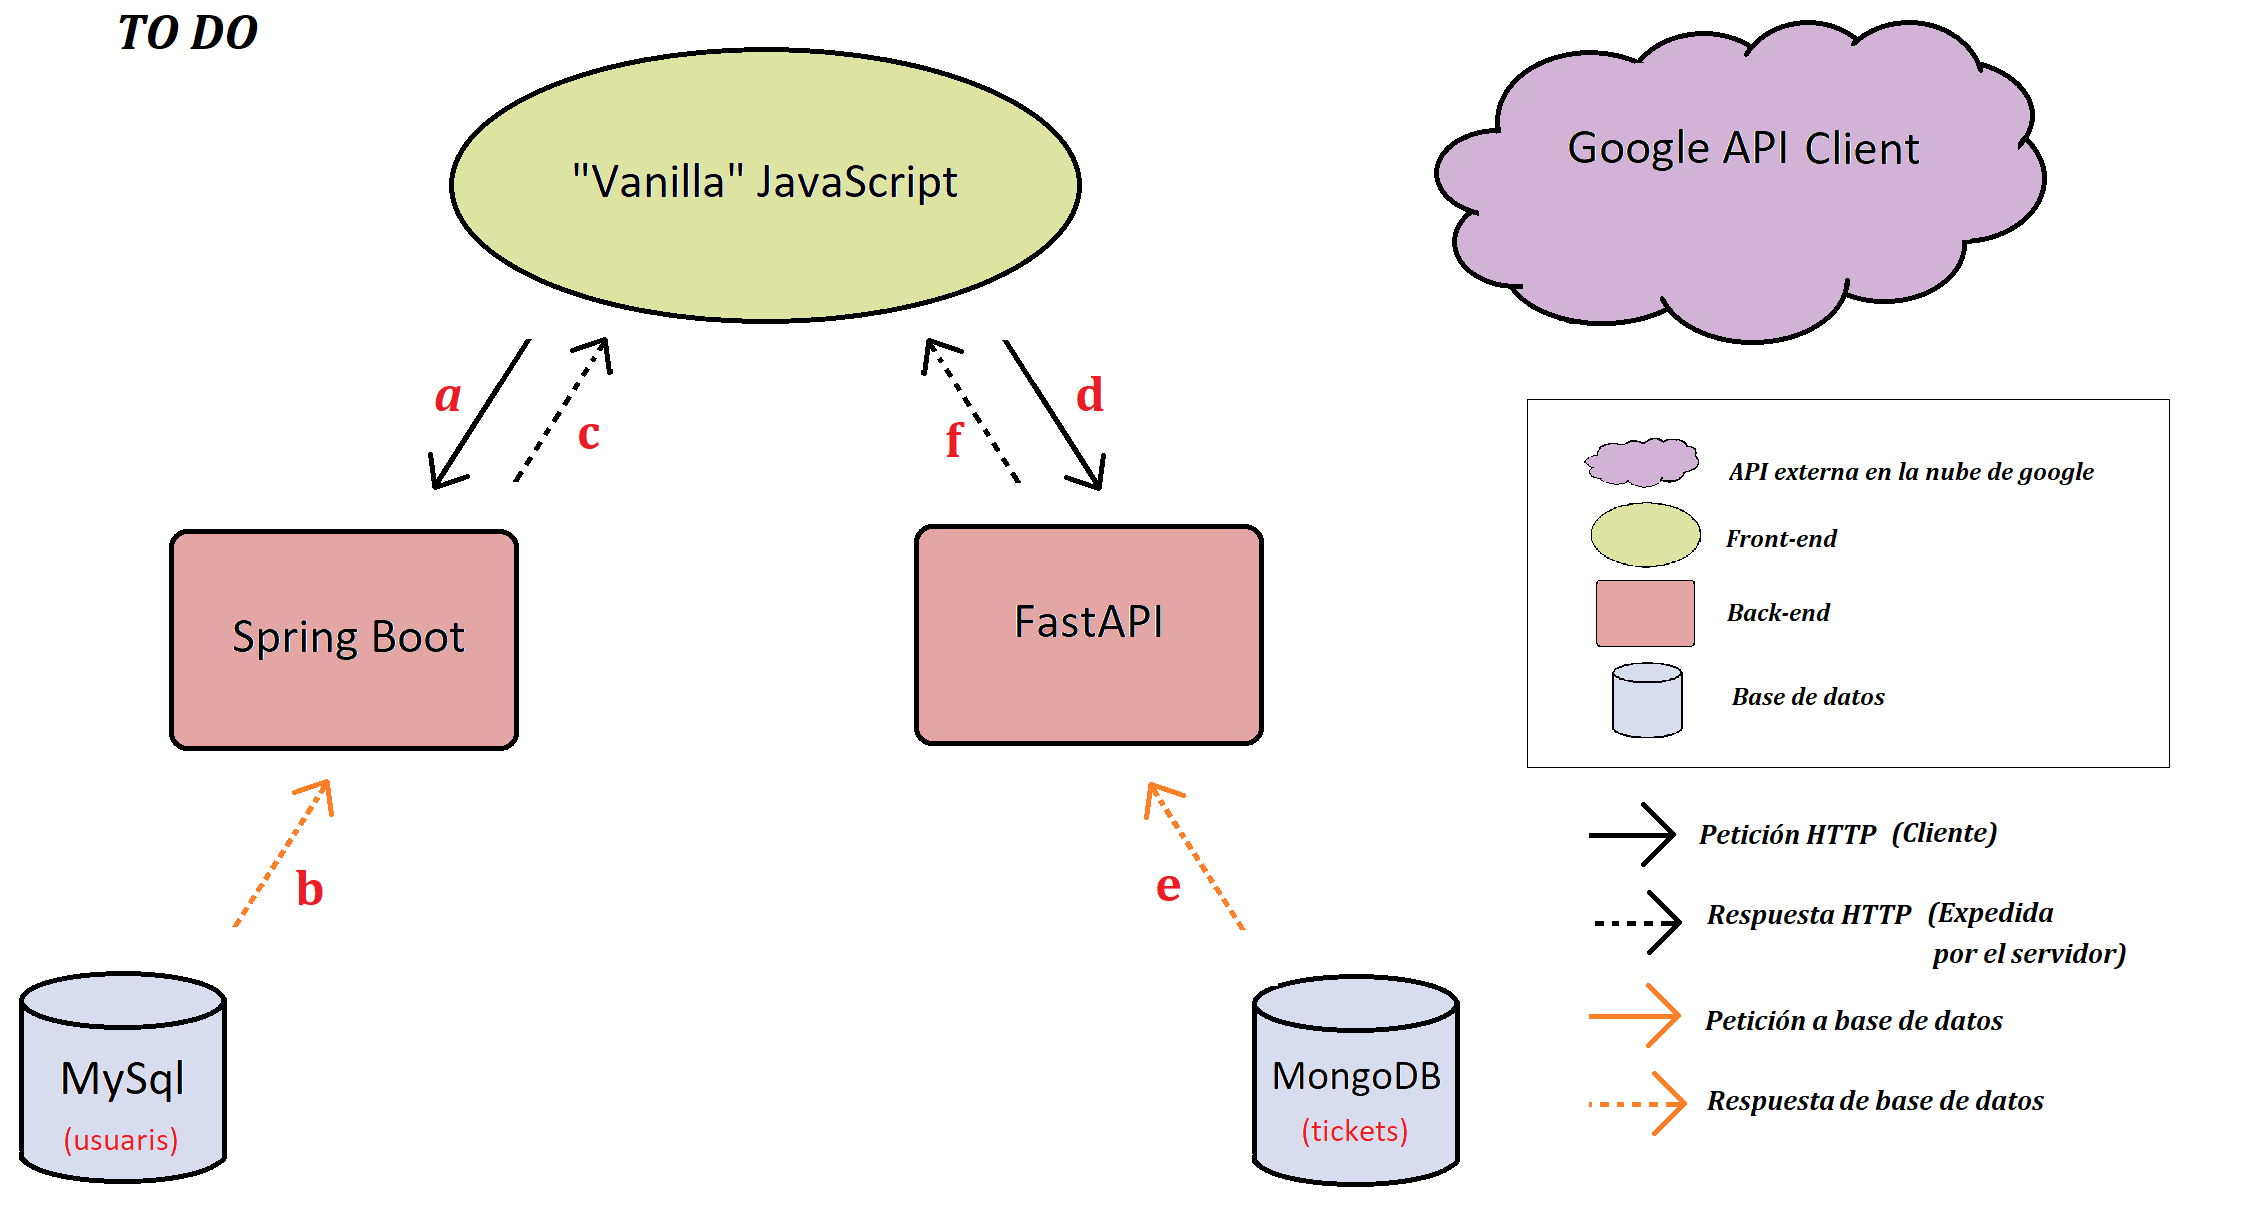
\includegraphics[width=1\linewidth]{../img/diagramaSistemesAplicacioMercappCAMIINICISESSIO}
			
			\label{fig:diagramasistemesaplicaciomercappcamiinicisessio}
		\end{figure}
		
	\end{frame}
	
	% Sección 3
	\section{Desarrollo}
	
	\begin{frame}
		\frametitle{Contenerización}
		Se ha automatizado la creación de imágenes y instanciado de contendores para cada microservicio
	
	\end{frame}
	
	% Sección 4
	\section{Conclusiones}
	
	\begin{frame}
		\frametitle{Conclusiones}
		\begin{itemize}
			\item Se ha aprendido a manejar tokens JWT
			\item etc etc
		\end{itemize}
	\end{frame}
	
	% Agradecimientos
	\begin{frame}
		\frametitle{Gracias por vuestra atención}
		¿Preguntas?
	\end{frame}
	
\end{document}
